\section{替代市场的修订结果}
本章使用上证50与纳斯达克综合指数评价相同模型家族，并增加XGB-AR对照。上证50在特征构造前删除2018年6月18日已确认休市行，修订样本为1500/500/1919；纳斯达克保持2000/500/1554。上证50采用中国月度EPU，纳斯达克采用美国月度EPU，真实发布时间与历史修订版本均未完整保存。不同市场与训练长度限制横向解释，不能称为独立外部验证。

\subsection{修订的点预测结果}
\begin{table}[htbp]\centering\caption{上证50日历修正后的结果，N=1919}\label{tab:sse50_metrics}
\begin{tabular}{lrrr}\toprule
模型 & MSE & MAE & QLIKE \\
\midrule
HAR & 4.826226 & 1.717026 & 3.872429 \\
GARCH(1,1) & 7.537442 & 2.043060 & 1.586804 \\
XGB-Market & 4.940740 & 1.740321 & 4.753901 \\
XGB-AR & 4.954984 & 1.741490 & 4.697720 \\
DEC & 4.972472 & 1.718639 & 3.672557 \\
\bottomrule\end{tabular}\end{table}
\begin{table}[htbp]\centering\caption{纳斯达克修订结果，N=1554}\label{tab:nas_metrics}
\begin{tabular}{lrrr}\toprule
模型 & MSE & MAE & QLIKE \\
\midrule
HAR & 5.292393 & 1.814872 & 3.994306 \\
GARCH(1,1) & 7.110225 & 1.894212 & 1.498305 \\
XGB-Market & 5.284620 & 1.767569 & 4.279836 \\
XGB-AR & 5.302560 & 1.761263 & 4.224645 \\
DEC & 5.369943 & 1.772158 & 3.895152 \\
\bottomrule\end{tabular}\end{table}

上证50中DEC相对XGB-Market和XGB-AR降低QLIKE及MAE，但提高MSE。纳斯达克中DEC相对两个XGB对照降低QLIKE，却同时提高MSE及MAE。三个市场的QLIKE排序均为GARCH最低，DEC其次，再是HAR及两个XGB对照中的其余模型；具体次序见完整表。加入EPU的收益依赖损失函数，不能声称跨指标普遍优势。

\subsection{纳斯达克规格改变及其原因}
历史单起点Beta解在299条估计残差上的SSE约1780.2771，验证MSE约4.3325。多起点找到训练SSE约1779.2408的更低解，但其验证MSE升至5.0476；此时12个月指数Almon的验证MSE为4.3446，成为六候选中的最小值。因此本文按原有选择规则改用Almon，而不是根据测试QLIKE选择Beta。

若强行固定历史12个月Beta规格、只修正求解，纳斯达克测试MSE为5.434646、QLIKE为3.791512；按验证规则重选Almon则为5.369943和3.895152。旧局部解可能产生类似隐式正则化的有限样本效果，但这只是解释假说，不能成为宣称已正确最小化训练目标的依据。更可靠的数值求解不保证更好的测试预测。

相对历史DEC的5.423666和3.794736，修订Almon的MSE下降约0.99\%，QLIKE上升约2.65\%。变化应如实报告，不选择性只展示有利指标。上证50包含数据清洗和求解两种变化，不能把历史表与修订表的总差值全部归因于优化器；项目另提供同输入的数值控制。
\subsection{上证50的图形结果}
\begin{figure}[H]\centering
\begin{minipage}{0.48\textwidth}\centering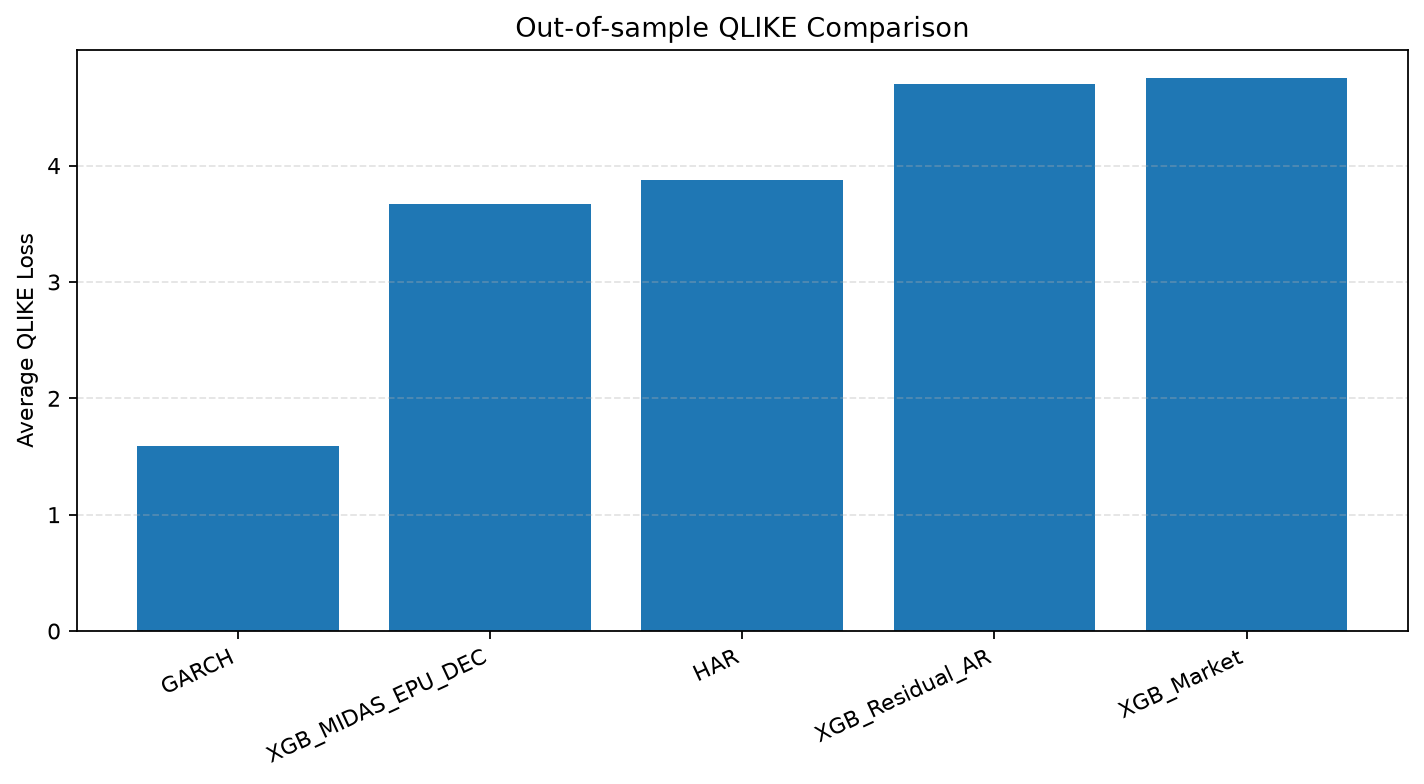
\includegraphics[width=\linewidth]{../../results/revised/sse50/fig_metrics_bar.png}\par{\small QLIKE}\end{minipage}\hfill
\begin{minipage}{0.48\textwidth}\centering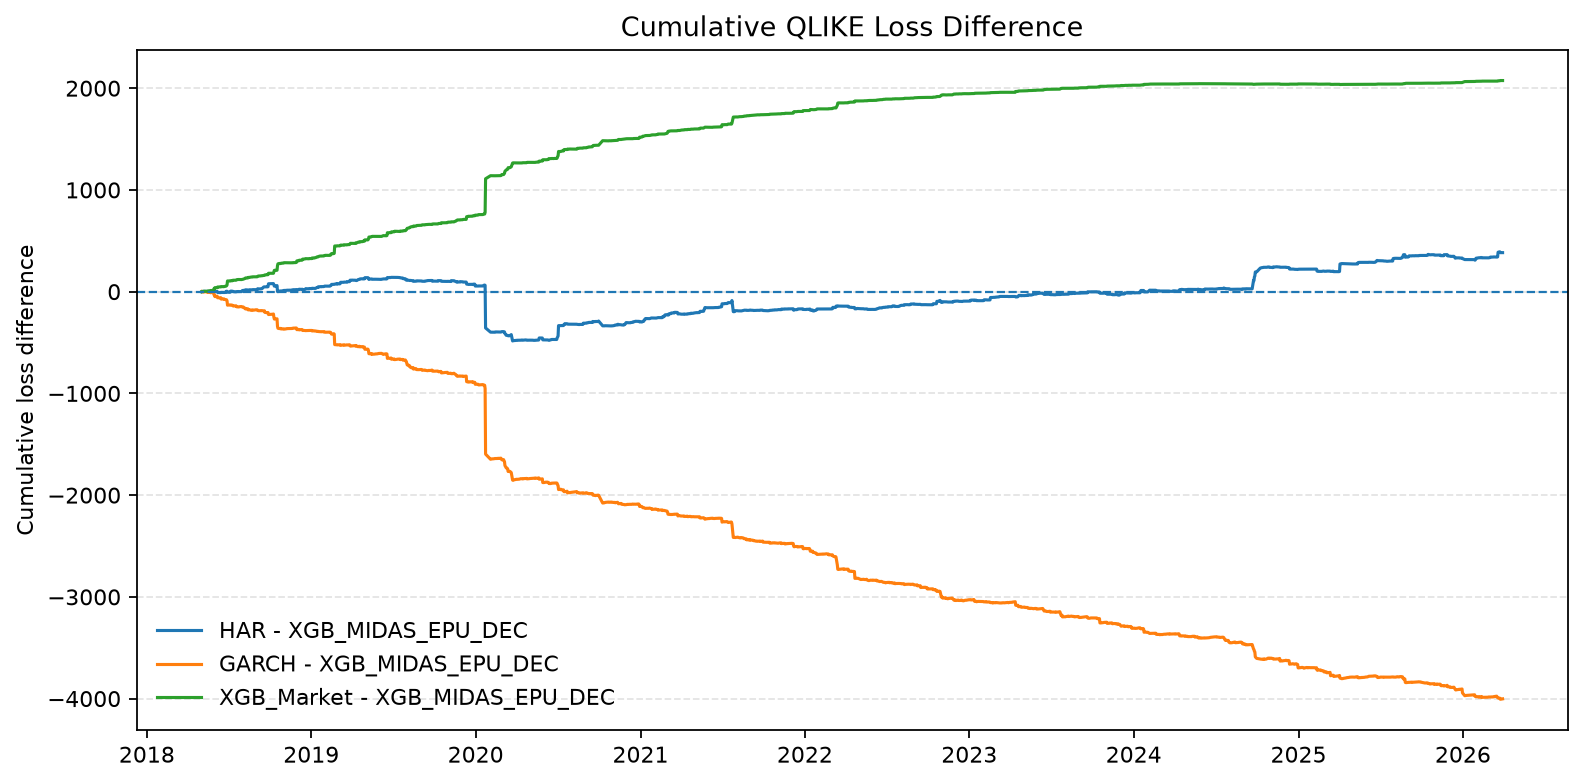
\includegraphics[width=\linewidth]{../../results/revised/sse50/fig_cumulative_qlike_diff.png}\par{\small 累计QLIKE差}\end{minipage}\par\medskip
\begin{minipage}{0.48\textwidth}\centering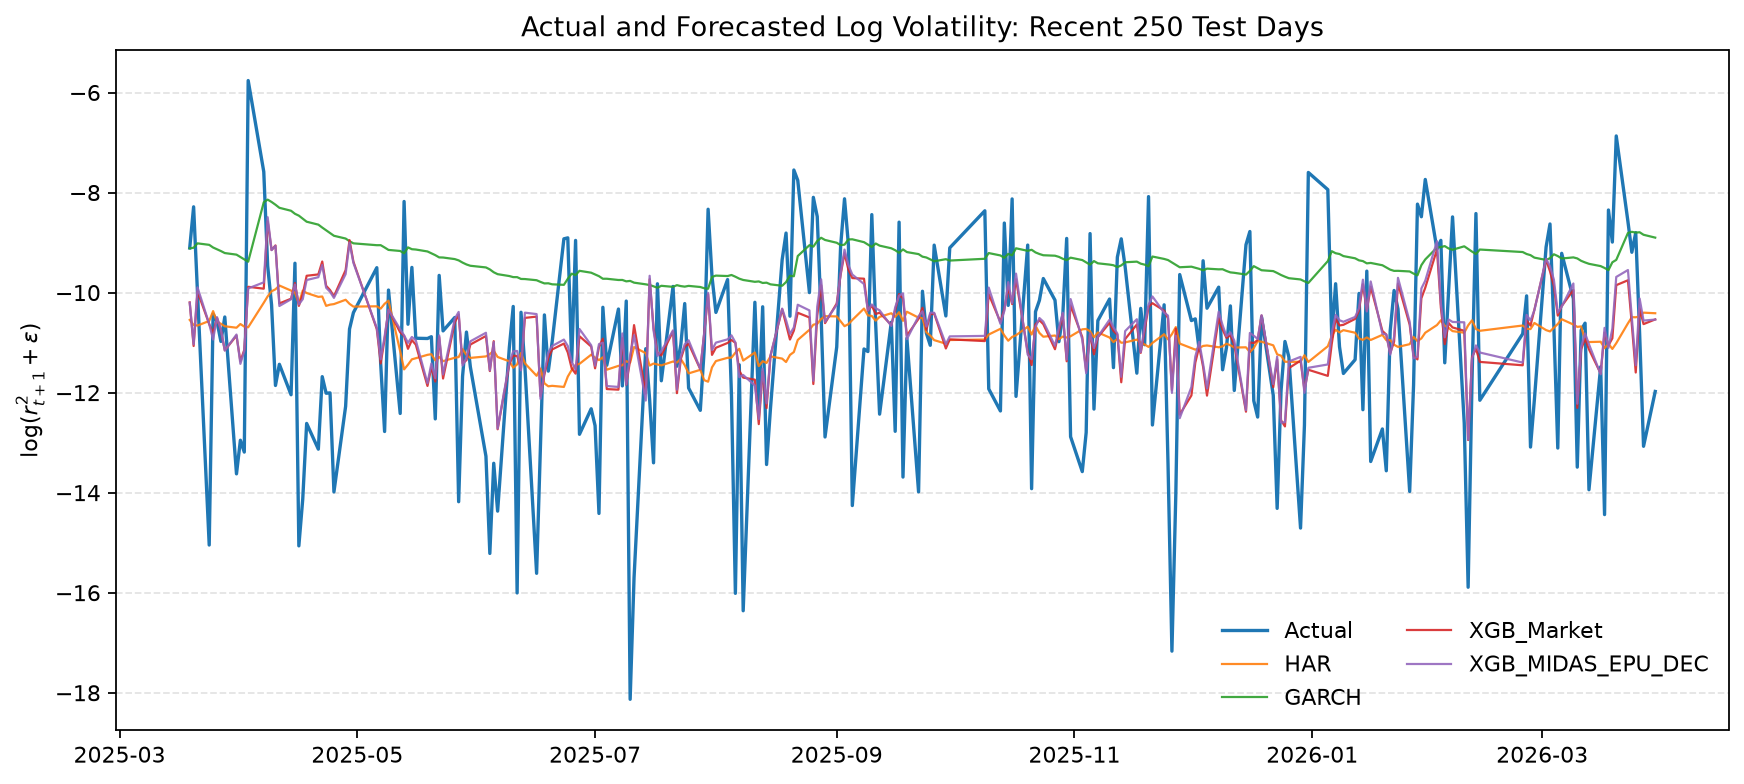
\includegraphics[width=\linewidth]{../../results/revised/sse50/fig_prediction_series_recent.png}\par{\small 近期预测}\end{minipage}\hfill
\begin{minipage}{0.48\textwidth}\centering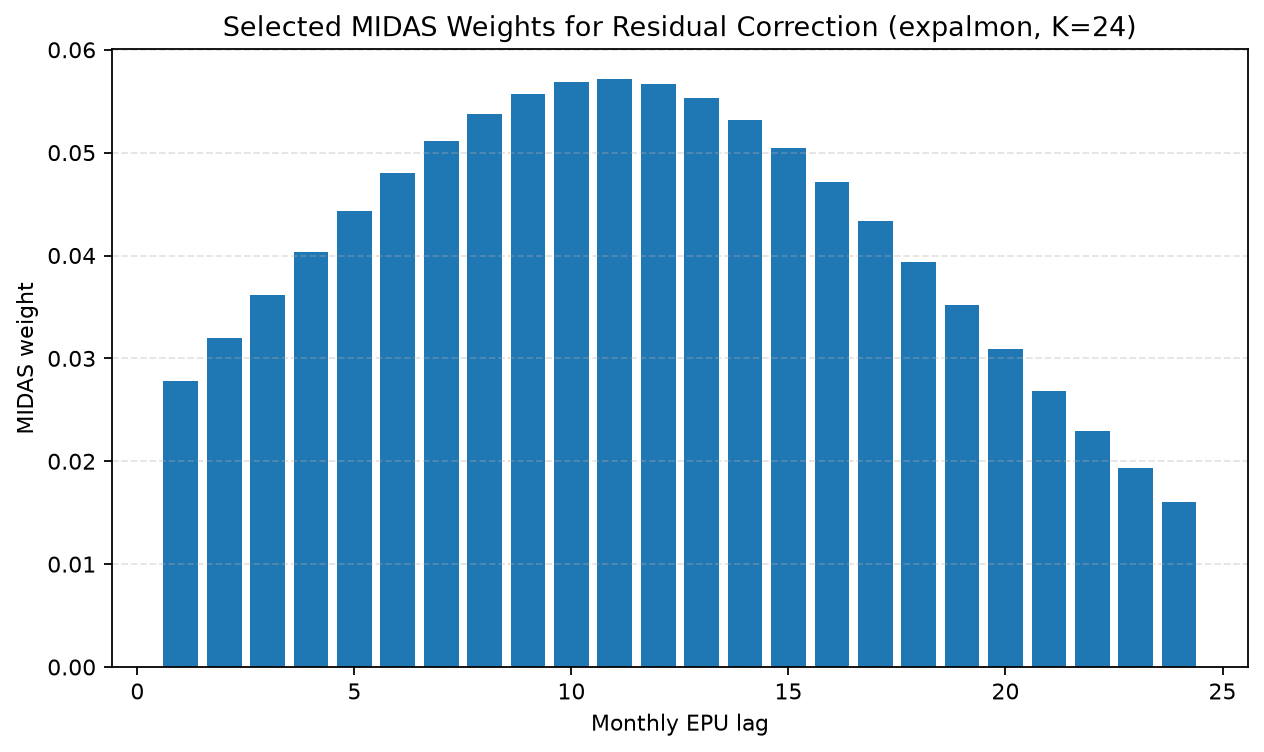
\includegraphics[width=\linewidth]{../../results/revised/sse50/fig_midas_weights.png}\par{\small 验证选择权重}\end{minipage}\par\medskip
\caption{上证50修订实验结果}\label{fig:sse50_robustness_panel}\end{figure}
\subsection{纳斯达克的图形结果}
\begin{figure}[H]\centering
\begin{minipage}{0.48\textwidth}\centering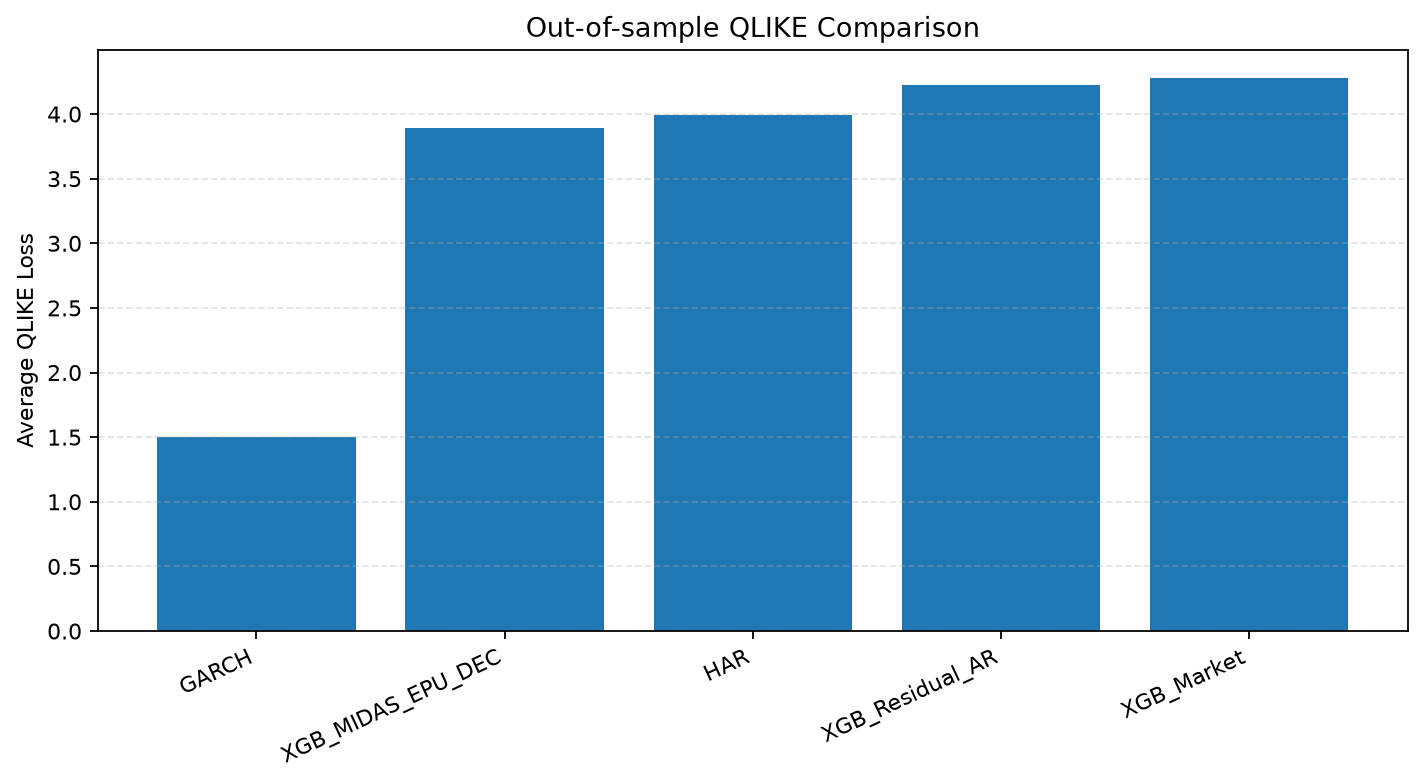
\includegraphics[width=\linewidth]{../../results/revised/nasdaq/fig_metrics_bar.png}\par{\small QLIKE}\end{minipage}\hfill
\begin{minipage}{0.48\textwidth}\centering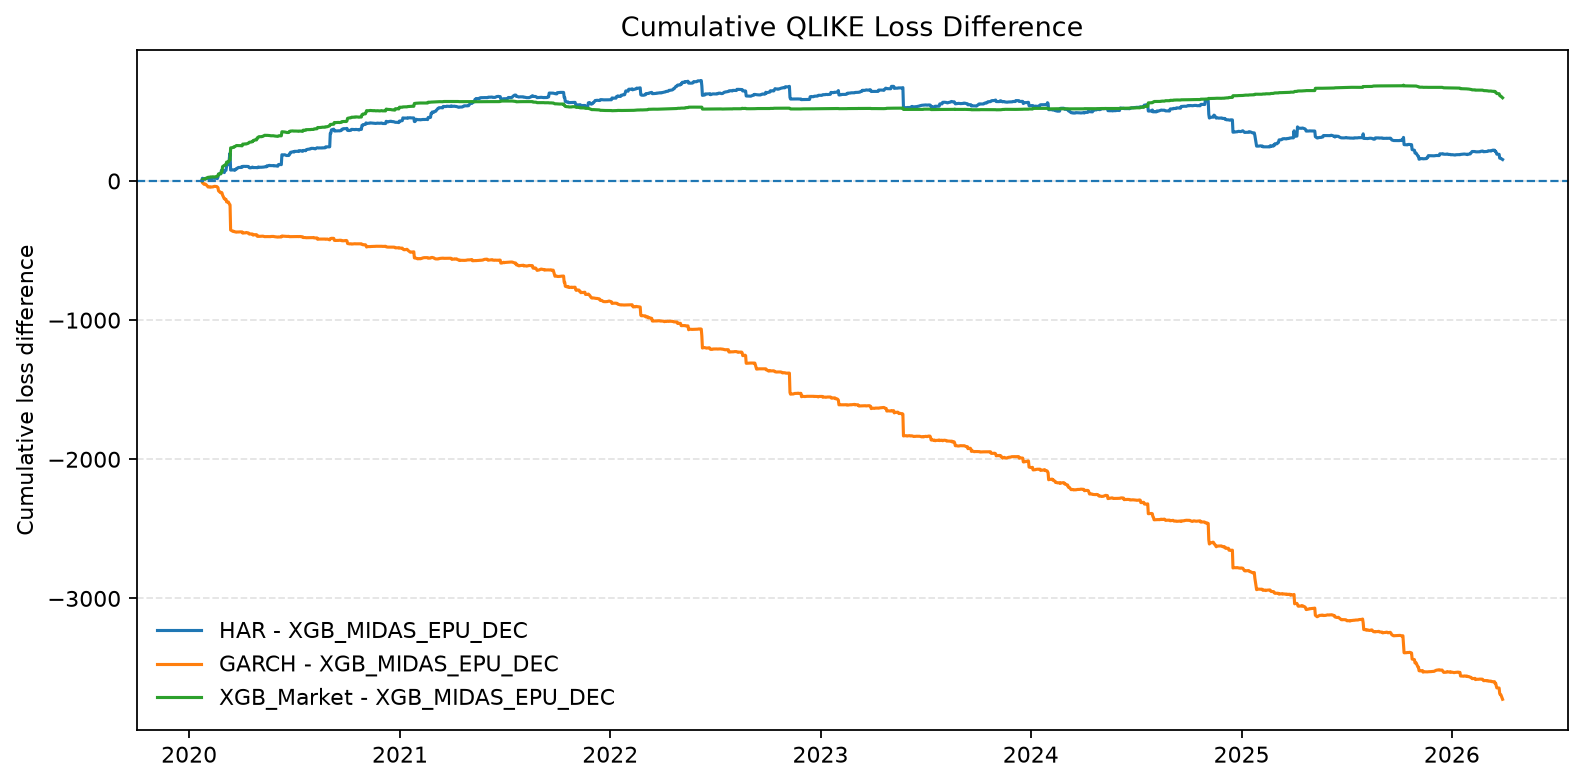
\includegraphics[width=\linewidth]{../../results/revised/nasdaq/fig_cumulative_qlike_diff.png}\par{\small 累计QLIKE差}\end{minipage}\par\medskip
\begin{minipage}{0.48\textwidth}\centering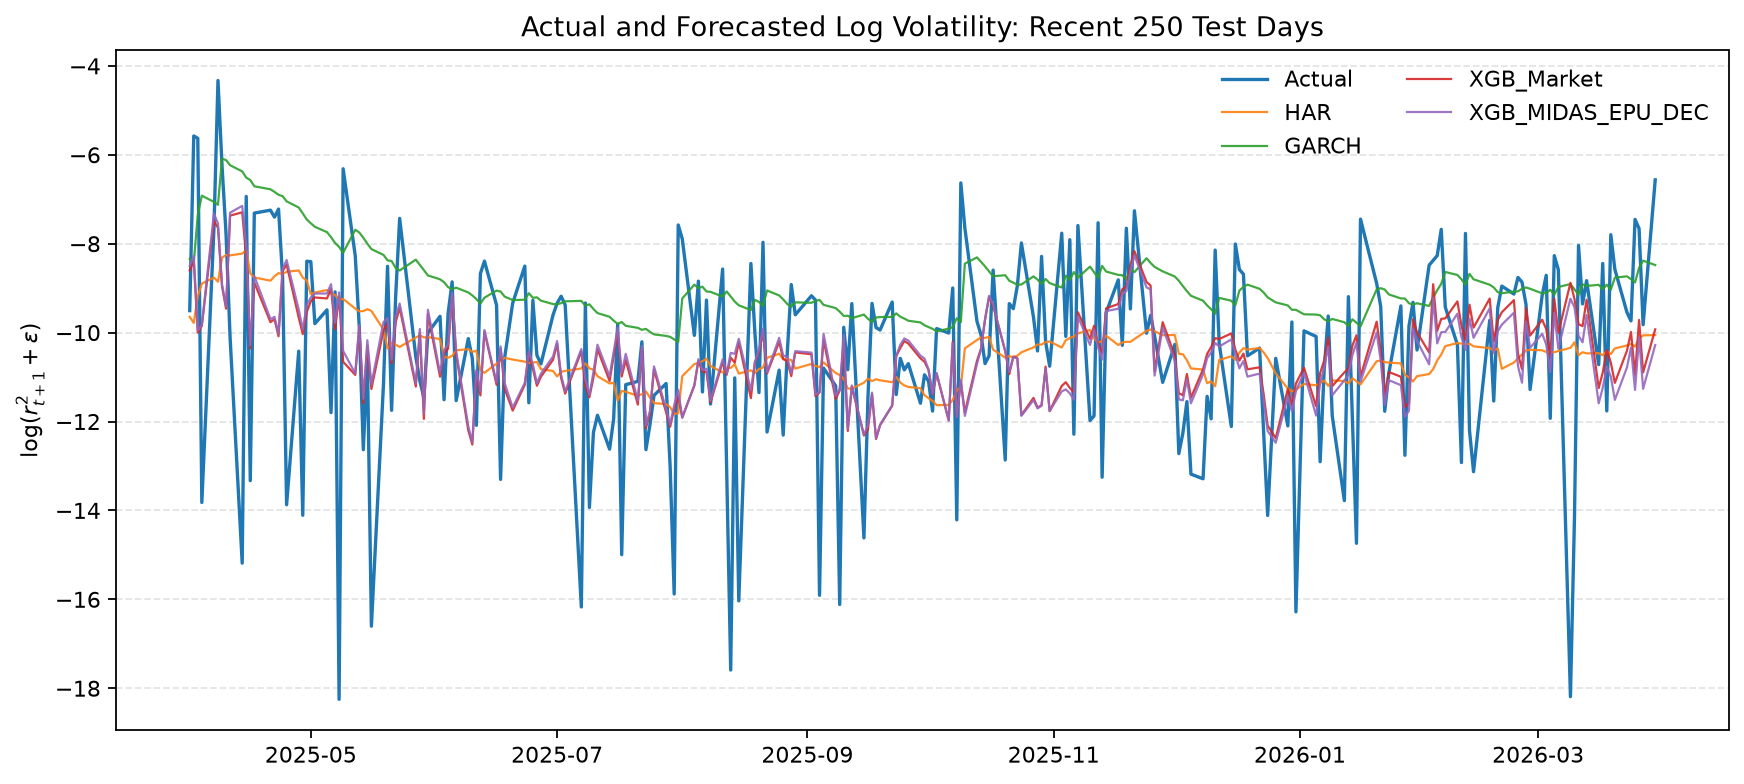
\includegraphics[width=\linewidth]{../../results/revised/nasdaq/fig_prediction_series_recent.png}\par{\small 近期预测}\end{minipage}\hfill
\begin{minipage}{0.48\textwidth}\centering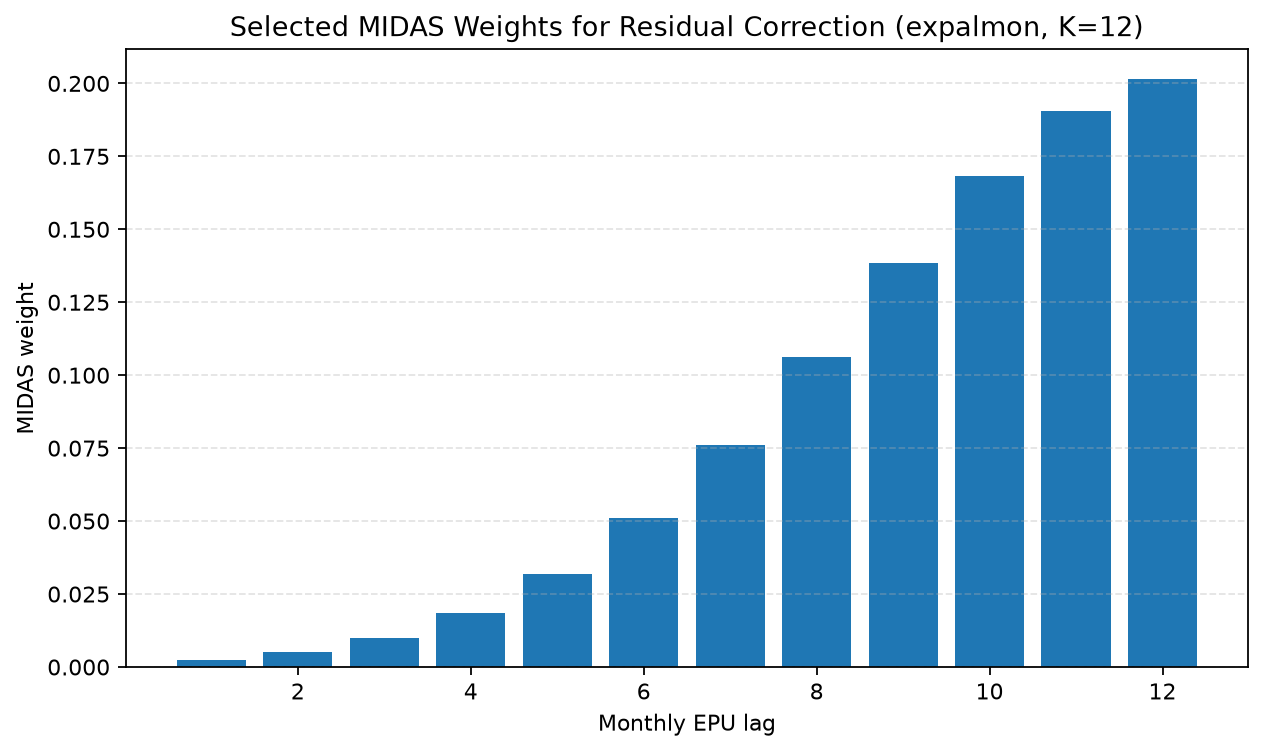
\includegraphics[width=\linewidth]{../../results/revised/nasdaq/fig_midas_weights.png}\par{\small 验证选择权重}\end{minipage}\par\medskip
\caption{纳斯达克修订实验结果}\label{fig:nas_robustness_panel}\end{figure}
\subsection{消融结果及解释范围}
三市场DEC相对XGB-AR的QLIKE均值差分别为1.168972、1.025163和0.329494；18项Holm调整后的正态参考$p$值分别约为$6.61\times10^{-12}$、$4.65\times10^{-7}$及0.0215。这是在回顾性、近似嵌套与规格选择限制下的探索性支持，不能升级为确定的总体优势。三市场MSE均较XGB-AR高，调整后没有支持MSE改善的证据。

中国两市场仍选择24个月指数Almon，纳斯达克改选12个月指数Almon。权重图展示验证阶段参数，测试期间会重估，边界解不应被解释为稳定政策传导机制。下一步应使用事先锁定的设计、独立时间留出集和真实发布版本的EPU，评估这些差异是否持续。
